%% == Casio VZ Virtual Instrument =============================================
%%    A virtual replica of the Casio VZ-1/VZ-10M music synthesizer
%% 
%% Matthias Wolff, BTU Cottbus-Sentenberg
%% August 30, 2019
%% DOI 
%%
%% References:
%% [1] 
%%
\documentclass[a4paper]{article}
%
% Packages
\usepackage{amsmath}
\usepackage{amssymb}
\usepackage[dvipsnames]{xcolor}
\usepackage{xspace}
\usepackage{authblk}
\usepackage[capitalize]{cleveref}
\usepackage{url}
\usepackage{tikz}
\usepackage{subcaption}
\usepackage{booktabs}
%
% Names
%\newcommand{\Ntikz}{TikZ\xspace}
%
% Custom commands
\newcommand\e{\mathrm{e}}
\renewcommand\i{\mathrm{i}}
\newcommand\person[1]{\textsc{#1}}
\newcommand{\TT}[1]{\protect\scalebox{0.75}[1.04]{\texttt{#1}}}
\newcommand\REMARK[1]{\vspace*{3pt}{%
  \setlength{\fboxrule}{0.5pt}%
  \setlength{\fboxsep}{3pt}
  
  \noindent\fbox{\begin{minipage}{0.985\textwidth}
  \textbf{Remark:} #1
  \end{minipage}}}\vspace*{3pt}
  
}
\newcommand{\CORR}[1]{{\color{red!90!RoyalBlue}#1}}
\newcommand{\workOn}{\color{Salmon!80!black}}
\newcommand{\workOff}{\color{black}}
\newcommand{\TODO}[1]{%
  \fboxsep=1pt\fboxrule=1pt\fcolorbox{yellow}{white}{[\textbf{TODO:~}#1]}%
}
\newcommand{\CHECK}[1]{%
  \fboxsep=1pt\fboxrule=1pt\fcolorbox{yellow}{white}{#1}%
}
%
% Settings
% - Page layout
\renewcommand{\floatpagefraction}{.8}
\textheight242mm
\textwidth150mm
\marginparwidth28mm
\topmargin-15mm
\oddsidemargin0mm
\evensidemargin0mm
% - Other
%\setcounter{secnumdepth}{2}

%%%%%%%%%%%%%%%%%%%%%%%%%%%%%%%%%%%%%%%%%%%%%%%%%%%%%%%%%%%%%%%%%%%%%%%%%%%%%%%

\begin{document}
%
\author{Matthias Wolff$^{\text{\sf\,[0000--0002--3895--7313]}}$}
\affil{BTU Cottbus-Senftenberg}
\title{Casio VZ Virtual Instrument:\\
A replica of the Casio VZ-1/VZ-10M music synthesizer}
\maketitle

\bigskip\noindent
See \TT{https://github.com/matthias-wolff/Casio-VZ-virtual-instrument/blob/master/Casio-VZ-virtual-instrument.pdf}
for the latest version of this document.
\begin{center}
  \bigskip\bigskip
  \begin{minipage}{0.9\linewidth}
    \textbf{Abstract}

    \bigskip
In this project I try to rebuild the vintage Casio VZ-1/VZ-10M music synthesizer
in Reaktor 6 \cite{Reaktor6}. The primary goal is a fully functional player
which is compatible with MIDI editor/librarian software like Midi Quest
\cite{MidiQuest12} or the like. My workplan is
\begin{enumerate}   
  \item 
    make some debugging and development tools (waveform validator, envelope
    validator, etc.),
  \item
    reproduce the 8 core waveforms of VZ-1/VZ-10M (1x sine, 5x sawtooth-like
    waveforms created by Casio's Phase Distortion Modulation, 1x white noise, 1x
    pitch-sensitive narrow-band noise),
  \item
    implement the core sound engine (wavetable oscillators, phase and ring
    modulators, VCAs, oscillator circuits),
  \item
    implement control signal generators (amplitude envelope, key following,
    layering, parametric sensitivity characterisitcs, etc.),
  \item
    implement MIDI SysEx control capability, and
  \item
    reproduce the factory voice and operation libraries.
\end{enumerate}
I always strongly disliked the unpleasant---though most
characteristic---aliasing and analog noise of the VZ-1. Hence, I will not
attempt to reproduce this. Insofar, the remake is not intended to be perfect.

As a secondary goal I may want to reproduce the GUI of the original instrument.
This would be a nice-to-have, however not necessarily of much practical use.

  \end{minipage}
  \vfill
  \vfill
\end{center}
\clearpage

\tableofcontents
\clearpage

%%%%%%%%%%%%%%%%%%%%%%%%%%%%%%%%%%%%%%%%%%%%%%%%%%%%%%%%%%%%%%%%%%%%%%%%%%%%%%%

\section{Goals and Prerequisites}
In this project I try to rebuild the vintage Casio VZ-1/VZ-10M music synthesizer
in Reaktor 6 \cite{Reaktor6}. The primary goal is a fully functional player
which is compatible with MIDI editor/librarian software like Midi Quest
\cite{MidiQuest12} or the like. My workplan is
\begin{enumerate}   
  \item 
    make some debugging and development tools (waveform validator, envelope
    validator, etc.),
  \item
    reproduce the 8 core waveforms of VZ-1/VZ-10M (1x sine, 5x sawtooth-like
    waveforms created by Casio's Phase Distortion Modulation, 1x white noise, 1x
    pitch-sensitive narrow-band noise),
  \item
    implement the core sound engine (wavetable oscillators, phase and ring
    modulators, VCAs, oscillator circuits),
  \item
    implement control signal generators (amplitude envelope, key following,
    layering, parametric sensitivity characterisitcs, etc.),
  \item
    implement MIDI SysEx control capability, and
  \item
    reproduce the factory voice and operation libraries.
\end{enumerate}
I always strongly disliked the unpleasant---though most
characteristic---aliasing and analog noise of the VZ-1. Hence, I will not
attempt to reproduce this. Insofar, the remake is not intended to be perfect.

As a secondary goal I may want to reproduce the GUI of the original instrument.
This would be a nice-to-have, however not necessarily of much practical use.

\subsection{The VZ-1/VZ-10M Music Synthesizer}
\TODO{\ldots}

\subsection{The Reaktor 6 Modular DSP Lab}
\TODO{\ldots}
\cite{Reaktor6}

\subsection{The Midi Quest 12 Editor/Librarian Software}
\TODO{\ldots}
\cite{MidiQuest12}

%%%%%%%%%%%%%%%%%%%%%%%%%%%%%%%%%%%%%%%%%%%%%%%%%%%%%%%%%%%%%%%%%%%%%%%%%%%%%%%

\section{Development and Debugging Tools}
\subsection{Waveform Validator}
\TODO{\ldots}

\subsection{Envelope Validator}
\TODO{\ldots}

%%%%%%%%%%%%%%%%%%%%%%%%%%%%%%%%%%%%%%%%%%%%%%%%%%%%%%%%%%%%%%%%%%%%%%%%%%%%%%%

\section{Development and Debugging Tools}

%%%%%%%%%%%%%%%%%%%%%%%%%%%%%%%%%%%%%%%%%%%%%%%%%%%%%%%%%%%%%%%%%%%%%%%%%%%%%%%

\section{Core Sound Engine}
VZ's sound engine is called ``iPD (interactive phase distortion) modular sound
engine'' \cite[p.\,12]{VZ1Manual}. According to Casio, this is an enhanced
version of the phase distortion modulation introduced by the predecessor of the
VZ-1 called CZ-1 \cite[p.\,39]{FS89}. Actually, the VZ synths series seem to
feature wavetable oscillators---with waveforms partly generated by the original
PD synthesis---together with ordinary phase modulation and ring modulation.

\subsection{Theory}
I assume that the reader is familiar with the basics of signal processing.
Introductions can be found in \cite{HW14} and \cite{OS14}.

\subsubsection{Tones, Timbre, Frequency, and Pitch}
A musical tone is a periodic sound. \cref{fig:MtSine} shows an example of the
most basic musical tone, a sine. Its mathematical representation is
\begin{equation}
  \label{eqn:MtSine}
  x(t) = a\sin(2\pi f_0 t+\varphi_0),
\end{equation}
where $a$ denotes the amplitude, $f_0$ denotes the tone (or fundamental)
frequency, and $\varphi_0$ denotes a phase offset.

\REMARK{Throughout this report I will assume continuous time signals $x(t)$
which, unless stated otherwise, take real values in $-1\leq x(t)\leq 1$, even
though we actually talk about digital signals of course. However, this
simplification saves some notational trouble.}

\cref{fig:Mt3Sines} shows an example of another basic tone composed by the
mixture of three sine tones. The timbre of a musical tone can be described
mathematically by the coefficients of its \person{Fourier} series, i.e., the
amplitudes and phase offsets of sine tones with frequencies $f=n\cdot f_0$
constituting the composed tone (see, e.g., \cite[p.\,102--113]{HW14}). More
complex tones comprise aperodic components (noise) and varying timbre over time.
%
\begin{figure*}
  \centering
  \begin{subfigure}[t]{0.5\textwidth}
    \centering
    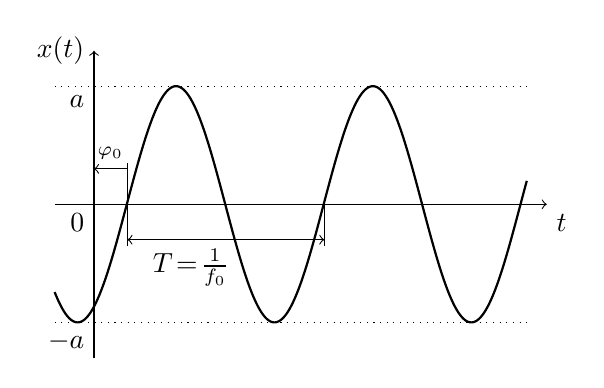
\begin{tikzpicture}[x=2.5cm, y=1.5cm]
      \draw[thin,->] (-0.2,0) -- (2.3,0) node[anchor=north west] {$t$};
      \draw[thin,->] (0,-1.3) -- (0,1.3) node[anchor=east] {$x(t)$};
      \node[anchor=north east] at (0,0) {$0$};
      \draw[thin,dotted] (-0.2, 1) -- (2.2, 1); \node[anchor=north east] at (0, 1) {$a$};
      \draw[thin,dotted] (-0.2,-1) -- (2.2,-1); \node[anchor=north east] at (0,-1) {$-a$};
      \draw[thick,smooth,samples=500,domain=-0.2:2.2,variable=\x] 
        plot ({\x},{sin(360*\x-60});
      \draw[thin]     (0.17, 0.35) -- (0.17,-0.35);
      \draw[thin]     (1.17, 0   ) -- (1.17,-0.35);
      \draw[thin,<->] (0.17,-0.3 ) -- (1.17,-0.3 );
      \draw[thin, ->] (0.17, 0.3 ) -- (0   , 0.3 );
      \node[anchor=north west] at (0.25,-0.3) {$T\!=\!\frac{1}{f_0}$};
      \node[anchor=south] at (0.083,0.3) {$\scriptstyle\varphi_0$};
    \end{tikzpicture}
    \caption{A sine tone\newline
      $x(t)=a\sin(2\pi f_0 t+\varphi_0)$
      \label{fig:MtSine}}
  \end{subfigure}~
  \begin{subfigure}[t]{0.5\textwidth}
    \centering
    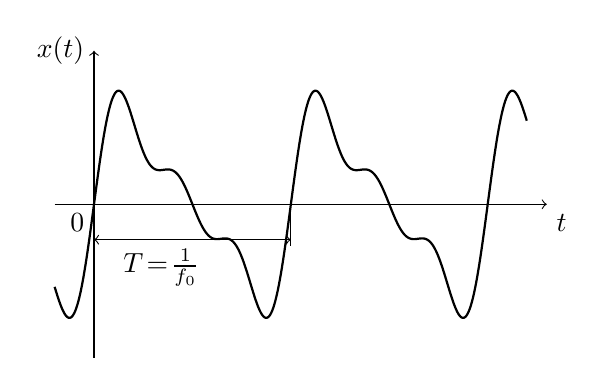
\begin{tikzpicture}[x=2.5cm, y=1.5cm]
      \draw[thin,->] (-0.2,0) -- (2.3,0) node[anchor=north west] {$t$};
      \draw[thin,->] (0,-1.3) -- (0,1.3) node[anchor=east] {$x(t)$};
      \node[anchor=north east] at (0,0) {$0$};
      \draw[thick,smooth,samples=500,domain=-0.2:2.2,variable=\x] 
        plot ({\x},{2/3*(sin(360*\x) + 1/2*sin(2*360*\x) + 1/3*sin(3*360*\x))});
      \draw[thin]     (1, 0   ) -- (1,-0.35);
      \draw[thin,<->] (0,-0.3 ) -- (1,-0.3 );
      \node[anchor=north west] at (0.1,-0.3) {$T\!=\!\frac{1}{f_0}$};
    \end{tikzpicture}
    \caption{A tone composed of three sines \newline
      $x(t)=\frac{2}{3}\sum\nolimits_{n=1}^2 \frac{1}{n}\sin(2\pi n f_0 t)$
      \label{fig:Mt3Sines}}
  \end{subfigure}
  \caption{Examples for basic musical tones. The tone frequency---measured in
  Hertz---is denoted by $f_0$. We denote time by $t$ and the duration of one
  cycle by $T$. Both are measured in seconds. The argument of the sine functions
  are called phase angles $\varphi$. One cycle corresponds to a phase difference
  of $\Delta\varphi = 2\pi$.}
\end{figure*}

As human perception of sound frequency is nearly logarithmic, Western music
theory commonly uses the pitch
\begin{equation}
  \label{eqn:f2p}
  p = 1200\cdot\log_2\!\left(\dfrac{f_0}{f_{\text{a}^1}}\right)
\end{equation}
measured in Cents (ct). The quantity in the denominator is a reference
frequency. I will use the concert pitch $f_{\text{a}^1}=440\,$Hz. Musical
intervals can be measured in terms of pitch. E.g., a semitone spans $100$\,ct, a
fith spans $500$\,ct, and an octave spans $1200$\,ct. Solving \cref{eqn:f2p}
for $f_0$, we obtain a formula for converting pitch to frequency:
\begin{equation}
  \label{eqn:p2f}
  f_0 = f_{\text{a}^1}\cdot 2^{\frac{p}{1200}}.
\end{equation}

\subsubsection{Phase Distortion Modulation}
% Macros for drawing PD characteristic curve -->
\newcommand\PDMcharact[3]{{%
  \begin{scope}[shift={(#1,#2)}]
    \def\aI{#3}
    \def\xxI{1/(2*\aI)}
    \draw[thick,domain=0:\xxI,variable=\x] plot ({\x},{\a*\x});
    \draw[thick,domain=\xxI:1,variable=\x] plot ({\x},{(\a*\x+\a-1)/(2*\a-1)});
  \end{scope}
}}
\newcommand\PDMsine[3]{{%
  \begin{scope}[shift={(#1,#2)}]
    \def\aI{#3}
    \def\xxI{1/(2*\aI)}
    \draw[very thin,dashed,domain=0:1,variable=\x] plot ({\x},{0.5*sin(360*\x-90)});
    \draw[thick,domain=0:\xxI,variable=\x] plot ({\x},{0.5*sin(360*\a*\x-90)});
    \draw[thick,domain=\xxI:1,variable=\x] plot ({\x},{0.5*sin(360*((\a*\x+\a-1)/(2*\a-1))-90)});
  \end{scope}
}}
% <--
Phase distortion modulation was invented in the early 1980's by \person{I.
Tomita}, \person{Y. Takahashi} and collegues of Casio Computer Ltd \cite{Ger09}.
It is based on the characteristic curve shown in \cref{fig:PDMcc}
\cite[p.\,20--21]{CZ1manual}.
%
\begin{figure*}[h!]
  \centering
  \begin{subfigure}[t]{0.45\textwidth}
    \centering
    \begin{tikzpicture}[x=3cm, y=3cm]
      \def\a{2}; % a_min = 1; a_max = 2+sqrt(3) = 3.7321
      \def\xx{1/(2*\a)};
      %
      \draw[thin,->] (-0.2,0) -- (1.3,0) node[anchor=north west] {$\varphi$};
      \draw[thin,->] (0,-0.2) -- (0,1.3) node[anchor=east] {$\varphi_{\text{PD}}(\varphi)$};
      \node[anchor=north east] at (0,0) {$0$};
      %
      \draw[very thin,dashed] (0,0) -- (1,1);
      \PDMcharact{0}{0}{\a};
      \node[anchor=south east] at({\xx/2},0.25) {$f_1=a\varphi$\!\!\!\!};
      \node[anchor=south east] at({\xx+(1-\xx)/2},0.75) {$f_2=b\varphi+c$\!\!\!\!};
      %
      \draw[thin,dotted] ({\xx},0.5) -- ({\xx}  ,-0.05) node[below] {$\varphi_B$};
      \draw[thin,dotted] (1    ,1  ) -- ( 1     ,-0.05) node[below] {$2\pi$};
      \draw[thin,dotted] ({\xx},0.5) -- (-0.05  , 0.5 ) node[left] {$\pi$};
      \draw[thin,dotted] (1    ,1  ) -- (-0.05  , 1   ) node[left] {$2\pi$};
    \end{tikzpicture}
    \caption{Piecewise linear phase charateristics\label{fig:PDMcc}}
  \end{subfigure}
  \begin{subfigure}[t]{0.45\textwidth}
    \centering
    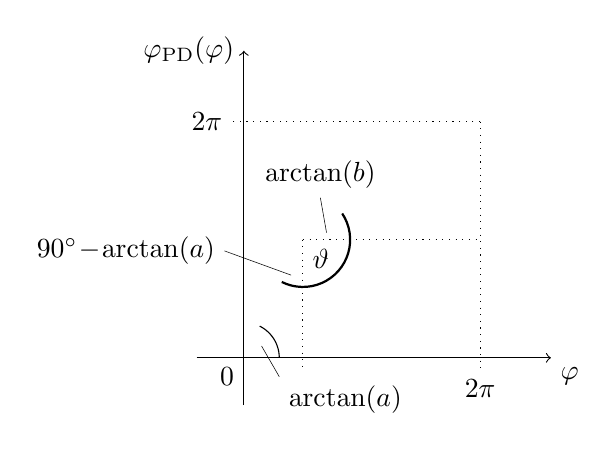
\begin{tikzpicture}[x=3cm, y=3cm]
      \def\a{2}; % a_min = 1; a_max = 2+sqrt(3) = 3.7321
      \def\b{\a/(2*\a-1)}
      \def\xx{1/(2*\a)};
      %
      \draw[thin,->] (-0.2,0) -- (1.3,0) node[anchor=north west] {$\varphi$};
      \draw[thin,->] (0,-0.2) -- (0,1.3) node[anchor=east] {$\varphi_{\text{PD}}(\varphi)$};
      \node[anchor=north east] at (0,0) {$0$};
      %
      \draw[domain=0:{atan(\a)},variable=\x] plot ({0.15*cos(\x)}, {0.15*sin(\x)});
      \draw[very thin] (0.075,0.05) -- +(-60:0.15) node[below right] {$\arctan(a)$};
      \draw[thick,domain={atan(\a)-180}:{atan(\b)},variable=\x] plot ({\xx+0.2*cos(\x)}, {0.5+0.2*sin(\x)});
      \node[anchor=north west] at ({\xx},0.5) {$\vartheta$};
      \draw[very thin] ({\xx-0.05},0.35) -- +(-200:0.3 ) node[left]  {$90^{\circ}\!-\!\arctan(a)$};
      \draw[very thin] ({\xx+0.1 },0.53) -- +( 100:0.15) node[above] {$\arctan(b)$};
      \PDMcharact{0}{0}{\a};
      %
      \draw[thin,dotted] ({\xx},0.5) -- ({\xx},-0.05);
      \draw[thin,dotted] ({\xx},0.5) -- (1    , 0.5 );
      \draw[thin,dotted] (1    ,1  ) -- (1    ,-0.05) node[below] {$2\pi$};
      \draw[thin,dotted] (1    ,1  ) -- (-0.05, 1   ) node[left]  {$2\pi$};
    \end{tikzpicture}
    \caption{Distortion angle $\vartheta$, $135^\circ\leq\vartheta\leq 180^\circ$\label{fig:PDMcc2}}
  \end{subfigure}
  \caption{Characteristic curve of phase distortortion}
\end{figure*}
We see that the curve consists of two straight sections
\begin{alignat}{5}
  f_1(\varphi) &= a\varphi, 
  & \quad 0&\leq\varphi <\varphi_B, 
  && \quad\text{connecting points } (0,0) \text{ and } (\varphi_B,\pi),\text{ and}
\\
  f_2(\varphi) &= b\varphi+c, 
  & \quad \varphi_B&\leq\varphi \leq 2\pi, 
  && \quad\text{connecting points } (\varphi_B,\pi) \text{ and } (2\pi,2\pi).
\end{alignat}
The slope $a$ of the first section is variable and can take real values $\geq
1$. The start and end points of the sections define the following constraints
\begin{alignat}{3}
  \label{eqn:PDMccc1}
  f_1(\varphi_B) &= a\varphi_B = \pi
  && \quad\leadsto \varphi_B = \frac{\pi}{a}
\\
  \label{eqn:PDMccc2}
  f_2(\varphi_B) &= \frac{\pi}{a}b + c = \pi
\\
  \label{eqn:PDMccc3}
  f_2(2\pi) &= 2\pi b + c = 2\pi
\end{alignat}
From \cref{eqn:PDMccc1,eqn:PDMccc2,eqn:PDMccc3} follows
\begin{equation}
  b = \frac{a}{2a-1}
  \quad\text{and}\quad
  c = \frac{2a-2}{2a-1}\pi,
\end{equation}
and finally
\begin{equation}
  \varphi_{\text{PD}}(\varphi)
  = \begin{cases}
      a\varphi
      & \text{for }0\leq\varphi < \frac{\pi}{a}
    \\[6pt]
      \dfrac{a\varphi+2\pi(a-1)}{2a-1}
      & \text{for }\frac{\pi}{a}\leq\varphi \leq 2\pi 
    \end{cases}
  \qquad\text{with }a\geq 1.
\end{equation}
Modulation depth can also be expressed by the angle between the straight
sections
\begin{equation}
  \label{eqn:PDMaToTheta}
  \vartheta/^{\circ} 
  = 180-\arctan(a)+\arctan(b)
  = 180-\arctan(a)+\arctan\!\left(\frac{a}{2a-1}\right)
\end{equation}
measured in degrees (see \cref{fig:PDMcc2}). Literature states that the
permissible range is $135^\circ\leq\vartheta\leq 180^\circ$ \cite{Ger09}.
However, for the wavetable of the VZ series this restriction does not seem to
hold. Measurement yielded angles down to $123^\circ$ corresponding to slope
parameters $a>10$ (see \TT{matlab/PDMwaves.mlx}). As I did not manage to solve
\cref{eqn:PDMaToTheta} for $a$, I just plot the function and print a lookup
table in \cref{fig:PDMaToTheta}.
%
\begin{figure*}
  \centering
  \begin{subfigure}{0.45\textwidth}
    \centering
    \begin{tikzpicture}[x=1cm, y=2cm]
      \def\offset{-120};
      \def\scale{1/45};
      \draw[thin,->] (-0.4,0) -- (5,0) node[anchor=north west] {$a$};
      \draw[thin,->] (0,-0.2) -- (0,1.5) node[anchor=east] {$\vartheta/^{\circ}$};
      \draw[thick,domain=1:5,variable=\x] plot ({\x},{(180-atan(\x)+atan(\x/(2*\x-1))+\offset)*\scale});
      \draw[thin,dotted] (1,{(180+\offset)*\scale}) -- (-0.2,{(180+\offset)*\scale}) node[left] {$180$}; 
      \draw[thin,dotted] (1,{(180+\offset)*\scale}) -- (1,-0.1) node[below] {$1$}; 
      \draw[thin,dotted] (3.73,{(135+\offset)*\scale}) -- (-0.2,{(135+\offset)*\scale}) node[left] {$135$}; 
      \draw[thin,dotted] (3.73,{(135+\offset)*\scale}) -- (3.73,-0.1) node[below] {$2\!+\!\sqrt{3}$}; 
    \end{tikzpicture}
    \caption{Distortion angle parameter $\vartheta$ as a function of slope parameter $a$}
  \end{subfigure}
  \begin{subfigure}{0.45\textwidth}
    \centering
    \begin{tabular}{llcll}\\ \toprule
      $\vartheta/^\circ$ & $a$ & & $\vartheta/^\circ$ & $a$  \\\midrule
      $135$ & $2\!+\!\sqrt{3}\approx 3.73$ && $160$ & $1.52$ \\
      $140$ & $2.92$                       && $165$ & $1.35$ \\
      $145$ & $2.39$                       && $170$ & $1.21$ \\
      $150$ & $2.02$                       && $175$ & $1.10$ \\
      $155$ & $1.74$                       && $180$ & $1.00$ \\\bottomrule \\
    \end{tabular}
    \caption{Lookup table}
  \end{subfigure}
  \caption{Relation between distortion angle parameter $\vartheta$ and slope
  parameter $a$, see \cref{eqn:PDMaToTheta}\label{fig:PDMaToTheta}}
\end{figure*}

Phase distortion modulation was applied in the Casio CZ synthesizer series.
\cref{fig:PDMCzExample} shows an example from the CZ manual. The VZ series uses
wavetables basing on PDM.
\begin{figure*}
  \centering
  \begin{subfigure}{0.3\textwidth}
    \centering
    \scalebox{0.65}{
      \begin{tikzpicture}[x=2cm, y=2cm]
        \def\a{1}; % a_min = 1; a_max = 2+sqrt(3) = 3.7321
        \def\xx{1/(2*\a)};
        %
        \draw[thin,->] (-0.2,0) -- (2.3,0) node[anchor=north west] {$\varphi$};
        \draw[thin,->] (0,-0.2) -- (0,1.3) node[anchor=east] {$\varphi_{\text{PD}}(\varphi)$};
        \node[anchor=north east] at (0,0) {$0$};
        \draw[thin,->] (-0.2,-1) -- (2.3,-1) node[anchor=north west] {$\varphi$};
        \draw[thin,->] (0,-1.7) -- (0,-0.3) node[anchor=east] {$\sin\!\left(\varphi_{\text{PD}}(\varphi)\!-\!\frac{\pi}{2}\right)$};
        %
        \PDMcharact{0}{0}{\a};
        \PDMcharact{1}{0}{\a};
        \PDMsine{0}{-1}{\a};
        \PDMsine{1}{-1}{\a};
        %
        \draw[thin] (0.05,-0.5) -- (-0.05,-0.5) node[left] {$1$};
        \draw[thin] (0.05,-1.5) -- (-0.05,-1.5) node[left] {$-1$};
        \node[anchor=north west] at (1,0) {\!$2\pi$};
        \node[anchor=north west] at (2,0) {\!$4\pi$};
        \draw[thin,dotted] ({\xx}  ,0.5) -- ({\xx}  ,-0.5);
        \draw[thin,dotted] ({1+\xx},0.5) -- ({1+\xx},-0.5);
        \draw[thin,dotted] (1      ,1  ) -- ( 1     ,-1.5);
        \draw[thin,dotted] ({1+\xx},0.5) -- (-0.05  , 0.5 ) node[left] {$\pi$};
        \draw[thin,dotted] (2      ,1  ) -- (-0.05  , 1   ) node[left] {$2\pi$};
        \draw[thin,dotted] (2      ,1  ) -- ( 2     ,-1.5);
      \end{tikzpicture}
    }
    \caption{$\vartheta=180^\circ$ ($a=1$)\newline no modulation}
  \end{subfigure}\hspace*{-3pt}
  \begin{subfigure}{0.3\textwidth}
    \centering
    \scalebox{0.65}{
      \begin{tikzpicture}[x=2cm, y=2cm]
        \def\a{2}; % a_min = 1; a_max = 2+sqrt(3) = 3.7321
        \def\xx{1/(2*\a)};
        %
        \draw[thin,->] (-0.2,0) -- (2.3,0) node[anchor=north west] {$\varphi$};
        \draw[thin,->] (0,-0.2) -- (0,1.3) node[anchor=east] {$\varphi_{\text{PD}}(\varphi)$};
        \node[anchor=north east] at (0,0) {$0$};
        \draw[thin,->] (-0.2,-1) -- (2.3,-1) node[anchor=north west] {$\varphi$};
        \draw[thin,->] (0,-1.7) -- (0,-0.3) node[anchor=east] {$\sin\!\left(\varphi_{\text{PD}}(\varphi)\!-\!\frac{\pi}{2}\right)$};
        %
        \draw[very thin,dashed] (0,0) -- (1,1);
        \draw[very thin,dashed] (1,0) -- (2,1);
        \PDMcharact{0}{0}{\a};
        \PDMcharact{1}{0}{\a};
        \PDMsine{0}{-1}{\a};
        \PDMsine{1}{-1}{\a};
        %
        \draw[thin] (0.05,-0.5) -- (-0.05,-0.5) node[left] {$1$};
        \draw[thin] (0.05,-1.5) -- (-0.05,-1.5) node[left] {$-1$};
        \node[anchor=north west] at (1,0) {\!$2\pi$};
        \node[anchor=north west] at (2,0) {\!$4\pi$};
        \draw[thin,dotted] ({\xx}  ,0.5) -- ({\xx}  ,-0.5);
        \draw[thin,dotted] ({1+\xx},0.5) -- ({1+\xx},-0.5);
        \draw[thin,dotted] (1      ,1  ) -- ( 1     ,-1.5);
        \draw[thin,dotted] ({1+\xx},0.5) -- (-0.05  , 0.5 ) node[left] {$\pi$};
        \draw[thin,dotted] (2      ,1  ) -- (-0.05  , 1   ) node[left] {$2\pi$};
        \draw[thin,dotted] (2      ,1  ) -- ( 2     ,-1.5);
      \end{tikzpicture}
    }
    \caption{$\vartheta=150^\circ$ ($a\approx 2$)\newline ~}
  \end{subfigure}\hspace*{-3pt}
  \begin{subfigure}{0.3\textwidth}
    \centering
    \scalebox{0.65}{
      \begin{tikzpicture}[x=2cm, y=2cm]
        \def\a{3.73}; % a_min = 1; a_max = 2+sqrt(3) = 3.7321
        \def\xx{1/(2*\a)};
        %
        \draw[thin,->] (-0.2,0) -- (2.3,0) node[anchor=north west] {$\varphi$};
        \draw[thin,->] (0,-0.2) -- (0,1.3) node[anchor=east] {$\varphi_{\text{PD}}(\varphi)$};
        \node[anchor=north east] at (0,0) {$0$};
        \draw[thin,->] (-0.2,-1) -- (2.3,-1) node[anchor=north west] {$\varphi$};
        \draw[thin,->] (0,-1.7) -- (0,-0.3) node[anchor=east] {$\sin\!\left(\varphi_{\text{PD}}(\varphi)\!-\!\frac{\pi}{2}\right)$};
        %
        \draw[very thin,dashed] (0,0) -- (1,1);
        \draw[very thin,dashed] (1,0) -- (2,1);
        \PDMcharact{0}{0}{\a};
        \PDMcharact{1}{0}{\a};
        \PDMsine{0}{-1}{\a};
        \PDMsine{1}{-1}{\a};
        %
        \draw[thin] (0.05,-0.5) -- (-0.05,-0.5) node[left] {$1$};
        \draw[thin] (0.05,-1.5) -- (-0.05,-1.5) node[left] {$-1$};
        \node[anchor=north west] at (1,0) {\!$2\pi$};
        \node[anchor=north west] at (2,0) {\!$4\pi$};
        \draw[thin,dotted] ({\xx}  ,0.5) -- ({\xx}  ,-0.5);
        \draw[thin,dotted] ({1+\xx},0.5) -- ({1+\xx},-0.5);
        \draw[thin,dotted] (1      ,1  ) -- ( 1     ,-1.5);
        \draw[thin,dotted] ({1+\xx},0.5) -- (-0.05  , 0.5 ) node[left] {$\pi$};
        \draw[thin,dotted] (2      ,1  ) -- (-0.05  , 1   ) node[left] {$2\pi$};
        \draw[thin,dotted] (2      ,1  ) -- ( 2     ,-1.5);
      \end{tikzpicture}
    }
    \caption{$\vartheta=135^\circ$ ($a\approx 3.73$)\newline resembling a sawtooth signal}
  \end{subfigure}
  \caption{Example of phase distortion modulation of the function
    $\sin\!\big(\varphi-\frac{\pi}{2}\big)$ adapted from 
    \cite[p.\,20--21, Figs.\,1--3]{CZ1manual}\label{fig:PDMCzExample}}
\end{figure*}

\REMARK{An alternate phase distortion characteristics $f(x)$ with
domain $0\leq x\leq 1$ taking values $0\leq f(x)\leq 1$ may be needed for
Reaktor implementation:
\begin{equation}
  f(x) = 
  \begin{cases}
    ax                   & 0\leq x < \frac{1}{2a}\\
    \dfrac{ax+a-1}{2a-1} & \frac{1}{2a} \leq x< 1
  \end{cases}
  \qquad\text{with }a\geq 1.
\end{equation}}

\subsubsection{Wavetable Osciallators}
The original VZ-1/VZ-10M is apparently based on wavetable oscillators
\cite[p.\,34]{VZ1Manual}. Such oscillators contain a set of digital waveforms,
each comprising exactly one signal period. Depending on the pitch, these
waveforms are played back at different rates. \TODO{\cref{fig:wavtab}} shows an
example of a VZ waveform (\TT{SAW4}).

Formally, a single waveform can be expressed by
\begin{equation}
  w(\varphi)\quad\text{with } 0\leq\varphi<2\pi,
\end{equation}
where the argument $\varphi$ is a phase angle. A oscillator based on this
waveform uses a time-varying phase angle $\varphi(t)$. Its output signal can be
written as
\begin{equation}
  \label{eqn:WavTabOsc}
  x(t) 
  = w\big(\varphi(t)\big)
  = w\big(2\pi (f_0t\!\!\!\mod 1)\big)\quad\text{with } -1\leq x(t)\leq 1
\end{equation}
where $w$ denotes a waveform, $f_0\in\mathbb{R}^{> 0}$ denotes the note
frequency in Hertz, and $t$ denotes the time in seconds. Further, we denote by
\begin{equation}
  x\!\!\!\mod 1 := x-\lfloor x\rfloor\quad\text{with } 0\leq (x\!\!\!\mod 1)<1
\end{equation}
the decimal fraction of the real valued quantity $x$. Hence, the argument
$\varphi(t) = 2\pi (f_0t\!\!\!\mod 1)$ on the right side of \cref{eqn:WavTabOsc}
involves resetting the phase angle of the waveform to zero whenever the cycle
length $2\pi$ is surpassed. \TODO{\cref{fig:WavTabOsc}} shows an example.

We will use the circuit symbol \TODO{\ldots} for a wavetable oscillator.

\subsubsection{Phase Modulation}

\subsubsection{Ring Modulation}

\subsection{VZ Hardware}
The VZ series features eight waveforms: sine (\TT{SINE}), five sawtooth-shaped
waveforms created by phase distortion modulation (\TT{SAW1}--\TT{SAW5}), white
noise (\TT{NOISE1}), and narrow-band noise (\TT{NOISE2}).

\subsection{Replica}
\subsubsection{Voltage-Controlled Oscillators (VCO)}

\subsubsection{Voltage-Controlled Amplifiers (VCA)}

%%%%%%%%%%%%%%%%%%%%%%%%%%%%%%%%%%%%%%%%%%%%%%%%%%%%%%%%%%%%%%%%%%%%%%%%%%%%%%%

\section{Control Signal Generators}

%%%%%%%%%%%%%%%%%%%%%%%%%%%%%%%%%%%%%%%%%%%%%%%%%%%%%%%%%%%%%%%%%%%%%%%%%%%%%%%

\section{MIDI SysEx Control}

%%%%%%%%%%%%%%%%%%%%%%%%%%%%%%%%%%%%%%%%%%%%%%%%%%%%%%%%%%%%%%%%%%%%%%%%%%%%%%%

%\pagebreak
\addcontentsline{toc}{section}{References}
\bibliographystyle{plain}
\bibliography{Casio-VZ-virtual-instrument}

\end{document}

%% EOF